\documentclass[10pt,letterpaper]{article}

\usepackage[margin=1in]{geometry}
\usepackage{iftex}
% mathptmx has no TU-encoded faces, so under XeTeX (Tectonic) earlier versions fell back
% to Latin Modern regular and lost every bold and italic. Use Termes there.
\ifPDFTeX\usepackage{mathptmx}\else\usepackage{fontspec}\setmainfont{texgyretermes}[Extension=.otf,UprightFont=*-regular,BoldFont=*-bold,ItalicFont=*-italic,BoldItalicFont=*-bolditalic]\fi
\usepackage{amsmath}
\usepackage{graphicx}
\usepackage{booktabs}
\usepackage{array}
\usepackage{listings}
\usepackage{xcolor}
\usepackage{tikz}
\usetikzlibrary{positioning,arrows.meta,fit,backgrounds,calc}
\usepackage{natbib}
\usepackage[colorlinks=true,linkcolor=blue,citecolor=blue,urlcolor=blue]{hyperref}
\usepackage{microtype}
\usepackage{parskip}
\usepackage{titlesec}
\usepackage{enumitem}
\usepackage{caption}
\usepackage{needspace}

\setlength{\parskip}{6pt}
\setlength{\parindent}{0pt}
\setlength{\emergencystretch}{3em}

\lstset{
  basicstyle=\small\ttfamily,
  breaklines=true,
  frame=single,
  numbers=left,
  numberstyle=\tiny,
  xleftmargin=2em,
  framexleftmargin=1.5em,
  backgroundcolor=\color{gray!8},
}

\definecolor{claimcolor}{RGB}{0,70,140}
\newcounter{claim}
\newenvironment{property}[1][]{%
  \refstepcounter{claim}%
  \needspace{6\baselineskip}%
  \vspace{4pt}%
  \noindent\fbox{\parbox{\dimexpr\linewidth-2\fboxsep-2\fboxrule}{%
    \textbf{\textcolor{claimcolor}{Property \theclaim} (#1).}
}}\par\vspace{2pt}%
}{\vspace{4pt}}

\title{\textbf{cA2A: Confidential Agent-to-Agent Delegation as a Profile on A2A}}

\author{
  Rishabh Poddar \quad Aaron Fulkerson \quad Imran Siddique \\
  OPAQUE Systems \\[4pt]
  \normalsize \url{https://github.com/agentrust-io/ca2a}
}

\date{October 1, 2026 \ \small Technical report, version 3}

\begin{document}

\maketitle

\begin{abstract}
The Agent2Agent (A2A) protocol moves tasks between agents, and its Signed Agent Card lets a
client check that a domain owner issued a card. The card does not bound the authority a
delegating agent passes on, establish what code a peer runs, keep a task payload from the
peer's host, or leave an offline record of who delegated what to whom. This technical report
describes cA2A (Confidential A2A), a trust profile layered on A2A rather than a new transport.
It composes four mechanisms: signed delegation credentials whose scope can only narrow at each
hop, appraisal of a peer's attestation evidence before a task is sent, a payload sealed to the
channel key that evidence vouches for, and a signed per-hop provenance record linked to its
parent. Attenuated delegation and provenance binding are covered by prior capability-token work
and IETF drafts; the contribution here is their composition on A2A with an open implementation.
We state six properties and report software experiments rerun against ca2a 0.3.1: attenuation
checks over 5,400 generated chains, rejection of in-chain replay and cross-chain splicing,
intersection of delegated scope with local policy, sealed-payload behavior at the cryptographic layer, structural checks on linked
provenance records, and a cross-operator attestation protocol exercised with synthetic
evidence. Chain verification cost about 0.22\,ms per hop in this environment. These results do
not show that a peer's key is confined to attested code or that attestation works across
independent operators. Recorded hardware runs cover one-directional appraisal of an Intel TDX
peer by an AMD SEV-SNP peer in another cloud and a same-operator mutual SEV-SNP diagnostic;
mutual attestation between independent operators has not been demonstrated.
\end{abstract}

\paragraph{Scope of this edition.}
This is an author-prepared technical report, not peer reviewed and not a normative
specification. Version 3 adds the caller-attestation relay that ca2a 0.4.0 fixed
(GHSA-xxj2-p57x-x954), which affects the release evaluated here, and corrects four statements:
0.3.1 was no longer the current release when version 2 appeared, a transparency log does not
make omission detectable, a wrong depth increment raises a broken-link error, and scope may stay
equal across a hop. It also restores bold and italic type that the Tectonic build had dropped. Results are unchanged. Version 2 (October 1, 2026) narrowed a design claim
of version 1 (September 27, 2026): the chain checks do not bind a delegation chain to a task or
execution, so a delegate can reuse a valid chain across tasks. Version 1 revised a draft dated
July 2026. Every software experiment was rerun on September 27, 2026 against ca2a 0.3.1 (commit
\texttt{7d90823}), then the current release; the July
results came from an unpinned earlier checkout and are retained beside the rerun. Correctness
counts are unchanged. Timings changed: chain verification rose from about 195 to about 216
microseconds per hop, and sealed-channel throughput at 256\,KiB fell from 266 to 212\,MiB/s.
Text, tables, and figures report the rerun. Status statements for C3 to C6 were revised to
match the 0.3.1 code, security fixes made after the original evaluation are reported in
Section~\ref{sec:after}, and the related work was corrected and extended. No hardware run was
repeated. Current behavior, requirements, and limitations are maintained in the project
repository.

\noindent\textbf{Patent Pending.}

\tableofcontents
\newpage

\section{Introduction}\label{sec:intro}

The Agent2Agent (A2A) protocol~\citep{a2a2026} defines how one agent discovers another and hands
it a task. It was contributed to the Linux Foundation, and on August 17, 2026 it joined the
Agentic AI Foundation as a hosted project, which reported backing from more than 150
organizations~\citep{aaifa2a2026}. Teams that need agents from different vendors to exchange work
increasingly have a common transport to build on.

A2A's trust anchor is the Signed Agent Card, which lets a client check that the owner of a
domain issued the card. It does not establish that a peer runs attested, unmodified code; that a
delegating agent actually holds the authority it passes on; that a task payload is confidential
to the intended peer; or that there is an auditable record of who delegated what to whom and
under which policy.

This gap matters once one agent delegates to another. Agent A hands a task to B, and B hands
part of it to C. Nothing in the transport constrains B or C to the authority A actually held. A
card-verified peer can request more than it was granted, and the request will look valid at every
hop. This is the confused deputy problem~\citep{confuseddeputy1988}, now across trust domains
that never negotiated a shared authority model. Recent work treats verifiable delegation for
agents as open: Prakash reports finding no prior implemented protocol that jointly combined
verifiable delegation, holder-side attenuation, chained policy, transport bindings, and provenance
records, and proposes one~\citep{aip2026}; Forough et al.\ list compound attestation for multi-hop
agent chains among the open challenges for confidential agentic AI~\citep{secretssurvey2026}.
Mutual TLS and OAuth scopes secure the connection and assert an identity; they do not attenuate
authority per hop, appraise runtime integrity, or seal a payload to an appraised peer.

This report describes cA2A (Confidential A2A), a trust \emph{profile} layered on A2A rather than a
competing transport. cA2A does not move tasks between agents; A2A does that. It defines the trust
envelope around a delegated task, in the way TRACE~\citep{trace2025} binds to
RATS~\citep{rats2021} and EAT~\citep{eat2023} rather than replacing them. cA2A composes four
mechanisms:

\begin{itemize}[leftmargin=1.5em]
  \item \textbf{Attenuated delegation.} Each hop carries a signed delegation credential whose
    scope is a subset of its parent's. Depth is bounded, the root issuer must be trusted by the
    verifier, and a credential identifier cannot repeat within a chain.
  \item \textbf{Runtime attestation.} A caller appraises a peer's attestation evidence, which
    binds the peer's channel key to a measurement, before it sends a delegated task.
  \item \textbf{Sealed peer channel.} The task payload is sealed to the channel key the appraised
    evidence vouches for, so only the holder of the matching private key can open it.
  \item \textbf{Provenance record.} Each hop emits a signed TRACE record referencing its parent
    record's hash and the delegation credential it acted under, so an auditor can check the
    path offline.
\end{itemize}

None of these mechanisms is new in isolation. Macaroons introduced offline attenuation of bearer
credentials~\citep{macaroons2014}, and recent agent-specific work specifies per-hop attenuation
with Cedar policies and parent-swap resistance~\citep{pedigree2026} or implements attenuated,
provenance-bound capability tokens across MCP and A2A~\citep{aip2026}. Section~\ref{sec:related}
compares them.

\subsection*{Contributions}

\begin{itemize}[leftmargin=1.5em]
  \item \textbf{The cA2A profile.} A binding on A2A, and on the IETF RATS, EAT, and
    SCITT~\citep{scitt2024} work, that composes attenuated delegation, attestation-gated sealing,
    and signed provenance for agent-to-agent calls without changing the A2A transport.
  \item \textbf{An open reference implementation.} The delegation credential model and offline
    chain verifier, the inbound decision path, the sealed channel, attestation verifiers for AMD
    SEV-SNP, Intel TDX, and TPM~2.0 evidence, signed TRACE provenance, and a CLI, released under
    the MIT license as ca2a-runtime~\citep{ca2arepo2026}. Delegation semantics mirror those of
    agent-manifest~\citep{agentmanifest2026}, and hardware-evidence parsing and certificate-chain
    checks are shared with it.
  \item \textbf{Six properties with their evidence stated.} We state six properties
    (Section~\ref{sec:claims}) and report software experiments rerun against ca2a 0.3.1
    (Section~\ref{sec:evaluation}). C1 (attenuation soundness) and C2 (in-chain replay and splice
    rejection) are validated in software. C3 (scope-policy intersection) is validated in software,
    including the inbound path of the reference transport. C4 (sealed-payload confidentiality) is
    validated at the cryptographic layer only. C5 (provenance integrity) is validated for
    structural consistency by the experiment, while authenticity rests on signed records covered by
    the project's tests. C6 (cross-operator attestation) is exercised with synthetic evidence and
    is not validated on hardware across independent operators.
\end{itemize}

\subsection*{Paper structure}

Section~\ref{sec:background} covers A2A and its Signed Agent Card, TEE attestation, the TRACE
record format, Cedar policy, and provenance. Section~\ref{sec:design} describes the cA2A profile
and how its mechanisms compose. Section~\ref{sec:claims} states the six properties and the status
of each. Section~\ref{sec:evaluation} presents the rerun experiments. Section~\ref{sec:after}
reports findings made after the original evaluation. Section~\ref{sec:related} surveys related
work, and Section~\ref{sec:conclusion} concludes.

\section{Background}\label{sec:background}

This section grounds cA2A in the protocols and mechanisms it composes. We describe A2A
and its Signed Agent Card, the tool-side analog in MCP and cMCP, capability attenuation
and how agent-manifest realizes a signed delegation chain, trusted execution environments
and remote attestation, the Cedar policy language, and the provenance and transparency
work that the TRACE record format draws on. None of this section is a novel claim; it
fixes terminology and states what each cited system provides.

\subsection{A2A and the Signed Agent Card}

The Agent2Agent (A2A) protocol~\citep{a2a2026} is a protocol for agent-to-agent
communication. An agent publishes an \emph{Agent Card}, a JSON document
that advertises the agent's identity, endpoint, and the skills it offers. A client agent
reads a peer's card, then sends it a \emph{task}, a unit of work the peer executes and
reports back on. A2A defines how tasks are moved and how their state transitions; it does
not define an authorization model for what a peer is permitted to do with a task once it
holds it.

The Signed Agent Card is A2A's trust anchor. The card carries a signature that lets a
client verify that the claimed domain owner issued it. This answers one question: did this
domain publish this card. It does not establish that the peer is running attested code,
that a delegating agent holds the authority it forwards, that the task payload is
confidential to the peer, or that there is an unbroken record of who delegated what to
whom. cA2A adds these guarantees as a profile on A2A rather than as a competing transport.

\subsection{MCP and cMCP as the Tool-Side Analog}

The Model Context Protocol (MCP)~\citep{mcp2024} standardizes how an agent discovers and
invokes tools hosted on external servers. Where A2A governs agent-to-agent calls, MCP
governs the agent-to-tool call. MCP, like A2A, defines discovery and invocation but not
authorization: it specifies no policy model, requires no audit record, and gives a client
no way to confirm that a cached tool definition is still the definition the server will
execute.

cMCP~\citep{cmcp2026} closes those gaps for the tool call. It interposes a gateway that
evaluates a Cedar policy per call, maintains a tamper-evident audit chain, and emits a
signed TRACE Claim that any verifier can check offline. cA2A is the agent-to-agent
counterpart of the same program: it takes the tool-side pattern of attested, policy-bound,
provable calls and applies it to the delegation edge between agents. cA2A reuses cMCP's
TEE provider pattern and runs the same Cedar engine (\texttt{cedarpy}) for local policy.

\subsection{Capability Attenuation and Macaroons}

The confused deputy problem~\citep{confuseddeputy1988} arises when a component with
authority is induced to exercise it on behalf of a caller who should not have that
authority. In a multi-agent workflow the deputy is any agent that accepts a narrow task
and then acts with broader authority than the task granted. The capability discipline
answers this by making authority a value that is passed explicitly and can only be
narrowed as it is passed on.

Macaroons~\citep{macaroons2014} are the reference construction for attenuable bearer
credentials. A macaroon is a token whose holder can append \emph{caveats} that restrict
its use, producing a strictly less powerful token without contacting the issuer; the chain
of caveats is bound by a keyed-HMAC construction so that no caveat can be dropped. The
essential property for delegation is monotone attenuation: a derived credential can only
be a subset of the one it derives from.

agent-manifest~\citep{agentmanifest2026} implements this discipline as a signed A2A
delegation chain. Each hop is a \texttt{DelegationCredential} whose signed body names the
issuer, the subject, the granted scope, a depth, and the parent hop's identifier. The body
is signed with Ed25519~\citep{eddsa2017} over a canonical JSON encoding aligned with RFC
8785~\citep{jcs2020}, so the exact bytes that were signed are reconstructable by any
verifier. Verification enforces signature validity at every hop, continuity of the
issuer-to-subject and parent-to-child links, a bounded depth, non-repetition of credential
identifiers to defeat replay, and the subset check on scope that enforces attenuation. cA2A
implements the same semantics in its own verifier, which the runtime calls on every inbound
peer request, and signs over RFC 8785 canonical bytes so that credentials are
cross-verifiable with agent-manifest. The attenuation subset check is what forecloses the
confused-deputy escalation.

\subsection{Trusted Execution Environments and Remote Attestation}

A Trusted Execution Environment (TEE) is a CPU-enforced isolation boundary that provides
two properties cA2A depends on: \emph{confidentiality}, so that memory inside the TEE is
inaccessible to software outside it including the hypervisor and host OS, and
\emph{remote attestation}, so that the TEE can produce a hardware-signed measurement report
proving to a remote verifier which code is running inside. AMD SEV-SNP~\citep{amdsevsnp2023}
and Intel TDX~\citep{inteltdx2023} are the two mainstream VM-level implementations; a survey
of confidential machine learning provides broader context~\citep{confai2024}.

The measurement report is the primitive of interest. Both platforms let the enclave place
application-chosen bytes into a report field bound to the hardware measurement, which is how
a public key can be tied to a specific attested measurement. The IETF RATS
architecture~\citep{rats2021} gives the vendor-neutral roles for this exchange, an attester
producing evidence and a verifier appraising it, and the Entity Attestation Token
(EAT)~\citep{eat2023} gives a portable token format for carrying attestation claims. cA2A
binds a peer's channel key to its attested measurement through this mechanism, so that a
caller can seal a payload to a key the appraised evidence vouches for. Whether that key is in
fact confined to the measured code depends on the platform and on what the measurement
covers; Sections~\ref{sec:claims} and~\ref{sec:after} state what has and has not been shown.

\subsection{Cedar Policy Language}

Cedar~\citep{cedar2023} is a policy language and evaluation engine that expresses access
control as \texttt{permit} and \texttt{forbid} rules over a principal, action, and
resource, with optional conditions over a context object. Cedar's structural typing keeps
evaluation decidable in bounded time, which matters when a policy check sits on the
critical path of accepting a delegated task. cA2A uses Cedar to model the intersection of a
forwarded delegation scope with a peer's local policy, so that a peer never acts beyond
either the authority delegated to it or its own operator's rules. Property~\ref{prop:c3}
states this intersection and Section~\ref{sec:eval-c3} evaluates it.

\subsection{Provenance and Transparency}

An offline-verifiable record of who delegated what to whom is a provenance problem. The
W3C PROV data model~\citep{prov2013} gives the vocabulary for describing entities,
activities, and the agents responsible for them, and the relationships that link a
derived artifact to what it was derived from. cA2A's per-hop records form a delegation DAG
in exactly this shape: each record names its parent, so the set of records across a
multi-hop workflow reconstructs the delegation tree.

A transparency log makes a registered record non-repudiable and lets anyone check that it was
included; it cannot reveal a record that was never registered. Certificate
Transparency~\citep{ct2013} established the pattern of an append-only, cryptographically
verifiable log for security-critical statements, and the IETF SCITT
architecture~\citep{scitt2024} generalizes it to supply-chain claims, giving neutral roles
for registering and auditing signed statements. cA2A follows the same profile-over-standard
posture toward SCITT that it takes toward A2A: it binds to the transparency architecture
rather than reinventing it.

\subsection{TRACE as the Record Format}

TRACE (Trust, Runtime Attestation, and Compliance Evidence)~\citep{trace2025} is the open
record format that cA2A emits per delegation hop. A TRACE record is a signed JSON document
that carries a subject, a runtime measurement, and profile-specific context. cA2A defines
an A2A profile of TRACE that adds a delegation-link block to each record: the hash of the
parent hop's record and the identifier of the delegation credential the hop acted under. A
root hop omits the block; every subsequent hop references its parent. Because each record
is signed and references its parent by hash, a verifier can rebuild the parent links,
confirm each hop acted under a credential whose chain verifies, and confirm that each record
was signed by the key the chain names as that hop's delegate. These checks run offline, given
the recipient's trusted keys and the delegation chain. They establish what the signers
declared, not that the declared work completed or that the submitted path is the complete
history, and the current verifiers accept one ordered root-to-leaf path rather than an
arbitrary branching graph. This is the record substrate for the provenance property in
Section~\ref{sec:claims}.

\section{Design}\label{sec:design}

\subsection{Profile, not protocol}

cA2A is a trust profile layered on the Agent2Agent (A2A) protocol \citep{a2a2026}, not a
competing transport. A2A moves tasks between agents and, through the Signed Agent Card,
answers exactly one question: did the domain owner issue this card. It does not establish
that a peer runs attested code, that a delegating agent actually holds the authority it
passes on, that a task payload is confidential to the intended peer, or that there is an
unbroken record of who delegated what to whom. cA2A adds that trust envelope around a
delegated task without redefining how the task is carried. It binds to A2A the way TRACE
\citep{trace2025} binds to the IETF RATS \citep{rats2021}, EAT \citep{eat2023}, and SCITT
\citep{scitt2024} work: as an overlay, not a replacement. The profile is written to be
independent of any one organization, cloud, or TEE vendor; the implementation currently
appraises AMD SEV-SNP, Intel TDX, and TPM~2.0 evidence.

Four design tenets constrain every primitive below. First, \emph{profile, not protocol}:
reuse A2A and the RATS, EAT, and SCITT stack rather than reinvent them. Second, \emph{neutral by
construction}: no coupling to a single silicon vendor, cloud, or model platform. Third,
\emph{fail closed}: absence of evidence is denial, not a warning; a missing attestation or an
unverifiable chain denies the call. Fourth, \emph{offline verifiable}: a third party can
verify a delegation chain and its provenance DAG without contacting or trusting any operator.

\subsection{Where cA2A attaches to A2A}

cA2A interposes on the trust decision that A2A leaves undefined: the moment one agent
receives a delegated task from a peer and must decide whether to accept it. On an inbound
peer call, the caller appraises the callee's attestation offer and seals the payload to the
channel key it vouches for. The callee then, in order, (i) verifies the delegation chain
(trusted root, signature, validity window, continuity, attenuation, in-chain replay, and
revocation when a snapshot is supplied), (ii) checks a holder proof showing that the caller
holds the key the chain delegates to, (iii) intersects the delegated scope with local policy,
(iv) appraises the caller's own attestation when the callee requires it, (v) decides the
requested capability, and (vi) only then opens the sealed payload and emits a linked
provenance record for the allow or deny decision. The A2A transport, agent identity issuance beyond delegation, and model governance
are all out of scope: cA2A governs only the delegation path between agents.

\subsection{Threat model}

cA2A defends the delegation path between agents against a capable adversary who may operate a
peer agent in a trust domain cA2A does not control; present a valid A2A Signed Agent Card
while running tampered or unmeasured code; sit on the network between two agents or operate
the host a peer runs on; and attempt to widen a delegated grant, replay a credential into
another chain, or reparent a provenance record. The assets and their defenses are summarized
in Table~\ref{tab:primitives}.

Out of adversary scope is breaking the underlying cryptographic primitives (Ed25519
\citep{eddsa2017}, the hash function) or compromising TEE firmware or hardware microcode
\citep{amdsevsnp2023,inteltdx2023}. Those are the trust anchors. The central attack cA2A
addresses is the confused deputy \citep{confuseddeputy1988} at machine speed: a delegate that
accepts a narrow task and then acts with authority it was never granted.

What ca2a 0.3.1 defends is narrower than this threat model. Attenuated delegation,
scope-policy intersection on the inbound path, the sealed channel's cryptography, and signed
provenance ship and are tested in software (Section~\ref{sec:evaluation}). Attestation
verifiers for SEV-SNP, TDX, and TPM evidence ship, and the live path can require hardware
assurance, but this is opt in: the reference client and server default to software assurance.
Hardware runs so far are one-directional across two clouds or mutual within one operator
(Section~\ref{subsec:attestation}). Confidentiality against a hosting operator additionally
depends on platform properties the recorded hosts lacked (Section~\ref{sec:after}). cA2A
should therefore not be described as attested across independent trust domains, and task
payloads should not be assumed protected from a hosting operator.

\subsection{Primitive 1: attenuated delegation}\label{subsec:delegation}

A delegation chain is a root-to-leaf list of signed credentials that lets Agent~A hand a
bounded slice of its authority to~B, and B a still-smaller slice to~C, with each grant
provably within the one above it. The semantics mirror the signed delegation chain
implemented and tested in agent-manifest \citep{agentmanifest2026}, and follow the
capability-attenuation model of macaroons \citep{macaroons2014}; cA2A implements that verifier
and its runtime calls it on every inbound peer request.

Each hop carries a \texttt{DelegationCredential} with a signed body and a detached Ed25519
signature. The body has \texttt{credential\_id} (a unique id for the hop), \texttt{issuer}
and \texttt{subject} (the delegator's and delegate's public keys), \texttt{scope} (the set of
capabilities granted at this hop), \texttt{depth} (0 at the root, $+1$ per hop),
and \texttt{parent\_id} (the parent hop's \texttt{credential\_id}, null at the root), with
optional \texttt{not\_before} and \texttt{not\_after} bounds. The signed bytes are the RFC~8785
\citep{jcs2020} canonical form of the body, with \texttt{scope} as a sorted array; floats are
refused and integers are bounded to the range RFC~8785 can represent exactly.

The verifier, \texttt{verify\_chain}, raises the specific error for the first invariant that
fails. The root issuer must be in the verifier's trusted set (else
\texttt{UNTRUSTED\_DELEGATION\_ROOT}); every hop's signature must verify against its issuer
(else \texttt{INVALID\_CREDENTIAL}) and its validity window must contain the evaluation time;
the root must have no parent and depth 0, each hop's \texttt{parent\_id} must equal the
previous hop's \texttt{credential\_id}, and each hop's \texttt{issuer} must equal the previous
hop's \texttt{subject}, and each hop's depth must be the previous depth $+1$ (else
\texttt{BROKEN\_DELEGATION\_LINK}); no depth may exceed \texttt{max\_depth} (else
\texttt{DELEGATION\_DEPTH\_EXCEEDED});
each hop's scope must be a subset of its parent's scope (else \texttt{SCOPE\_ESCALATION});
and no \texttt{credential\_id} may repeat (else \texttt{CREDENTIAL\_REPLAY}). Given a signed
revocation snapshot, a hop revoked by its issuer or any issuer above it is refused
(\texttt{CREDENTIAL\_REVOKED}). The verifier keeps no global history of used credentials, so
replay of a whole valid chain by a different party is addressed by the holder proof in the
inbound path rather than by \texttt{verify\_chain}.

Consider the chain
\[
  \text{A} \xrightarrow{\ S_A\ } \text{B} \xrightarrow{\ S_B \subseteq S_A\ } \text{C},
  \qquad S_C \subseteq S_B \subseteq S_A .
\]
A issues B a child credential whose scope $S_B$ is a subset of A's grant $S_A$, signed over
the canonical body. B in turn issues C a credential with $S_C \subseteq S_B$. The subset
check at every hop is the confused-deputy defense within a chain: it forecloses B accepting a narrow task
from A and then acting with authority A never granted. Attenuation is the whole point.
The \texttt{parent\_id}, \texttt{issuer}/\texttt{subject} continuity, and unique-id checks
close the complementary attack of replaying a credential within a chain or splicing one from
another chain into it. They do not bind a chain to a particular task or execution: a credential
carries no task or execution identifier, so the delegate can present the same valid chain
with a different request. Making execution lineage part of the authorization decision is the
subject of history-based access control \citep{abadi2003history}, provenance-based access control
\citep{park2012pbac}, and, for agent delegation, the PIC model \citep{gallo2026pic}. cA2A does not
provide it; authenticated lineage records (Section~\ref{sec:after}) say which hop acted under
which credential, which is not the same as refusing authority outside its lineage. This primitive is implemented and validated (Properties~\ref{prop:c1}
and~\ref{prop:c2}).

\subsection{Primitive 2: runtime peer attestation}\label{subsec:attestation}

Before a peer is trusted with a delegated task, it presents evidence of the code it runs. cA2A
follows the TEE provider pattern of cMCP \citep{cmcp2026}. A provider
implements \texttt{detect()}, returning whether it is available on the current host, and
\texttt{attest(public\_key, nonce)}, returning an \texttt{AttestationReport} that binds a
public key to the host's hardware measurement under a nonce. The report carries
\texttt{platform}, \texttt{measurement}, the bound \texttt{public\_key}, and the \texttt{nonce},
following the RATS evidence model \citep{rats2021} and EAT claims format \citep{eat2023}.

The providers are a \texttt{software-only} backend (for development and CI, which reports
\texttt{platform:\ software-only} and never a hardware platform string) and three hardware
backends: \texttt{tpm} (TPM 2.0 or vTPM), \texttt{sev-snp} (AMD SEV-SNP \citep{amdsevsnp2023}),
and \texttt{tdx} (Intel TDX \citep{inteltdx2023}).

\textbf{Implementation status at 0.3.1.} The SEV-SNP and TDX verifiers check certificate chains
to pinned AMD and Intel roots, report signatures, and key binding, and the project records runs
against genuine evidence from both platforms; for this edition the TDX verifier was re-run
against a public GCP TDX quote (Section~\ref{sec:evaluation}). The TPM verifier checks quote
structure, binding, and attestation-key signature; its certificate chain depends on a
caller-supplied vendor root, and on one Azure host generation no chain to a pinnable root could
be assembled. SEV-SNP and TDX collectors use the kernel configfs-TSM interface and have run on
GCP confidential VMs; an Azure SEV-SNP guest is paravisor-mediated, cannot set
\texttt{REPORT\_DATA} directly, and roots its channel key through the vTPM instead. The project
records two live runs. On July 27, 2026 an Azure SEV-SNP caller appraised a GCP TDX peer's quote
against the Intel root, sealed a delegated task to the bound key, and the peer allowed an
in-scope capability and refused an out-of-scope one; the callee did not appraise the caller, and
one operator ran both sides. On September 17, 2026 two GCP SEV-SNP guests in one project
appraised each other and exchanged sealed non-secret payloads in both directions. Neither run is
mutual attestation between independent operators, so Property~\ref{prop:c6} is not validated on
hardware. Verification fails closed when required evidence is absent. In 0.3.1 a required caller
appraisal could be satisfied by an offer relayed from another node (Section~\ref{sec:after}).

\subsection{Primitive 3: sealed peer channel}\label{subsec:sealed}

When A sends B a task payload, that payload crosses a network and lands in B's memory. If B is
in another trust domain, mTLS protects the pipe but not the endpoint: the operator hosting B,
or a connectivity provider between them, can read plaintext. The sealed channel encrypts the
payload to B's channel public key, and B's attestation evidence binds that key to a
measurement, extending the attestation-gated key pattern cMCP uses for the agent-to-gateway
case to the peer-to-peer case. The connectivity path sees ciphertext. The interface is
\texttt{SealedChannel(peer\_public\_key).seal} on the sender and \texttt{open\_sealed} with the
private key on the receiver.

\textbf{Cryptographic layer: implemented and validated.} The channel ships over
X25519 ECDH, HKDF-SHA256 key derivation, and ChaCha20-Poly1305 AEAD. A payload sealed to a
peer's channel key decrypts only with that key, the connectivity path sees only ciphertext, and
a tampered blob fails AEAD authentication so \texttt{open} fails closed rather than returning
plaintext. Property~\ref{prop:c4} validates exactly this at the cryptographic layer
(Section~\ref{sec:evaluation}).
\textbf{Binding to attestation.} On the live path the caller seals only to a channel key that
its verifier has appraised (\texttt{ca2a\_runtime.attestation}). In software mode that appraisal
has assurance \texttt{none}; with a hardware verifier configured and
\texttt{require\_hardware} set, a software offer is refused before sealing. Even with hardware
appraisal, the channel key is an ordinary key held by a process in the guest. In the
September 17 diagnostic the launch measurements did not cover application code installed after
boot, and the SEV-SNP hosts reported that ciphertext hiding was not enabled. Confidentiality
against the hosting operator therefore remains the dependency that Property~\ref{prop:c4}
names.

Figure~\ref{fig:sealed-channel} shows the seal-and-open path. The sender derives a
one-time symmetric key from an ephemeral X25519 ECDH to the peer's channel public key,
runs it through HKDF-SHA256, and encrypts the payload under ChaCha20-Poly1305. The
connectivity path sees only the sealed blob; only the holder of the peer's channel private key
recovers the plaintext.

\begin{figure}[h]
\centering
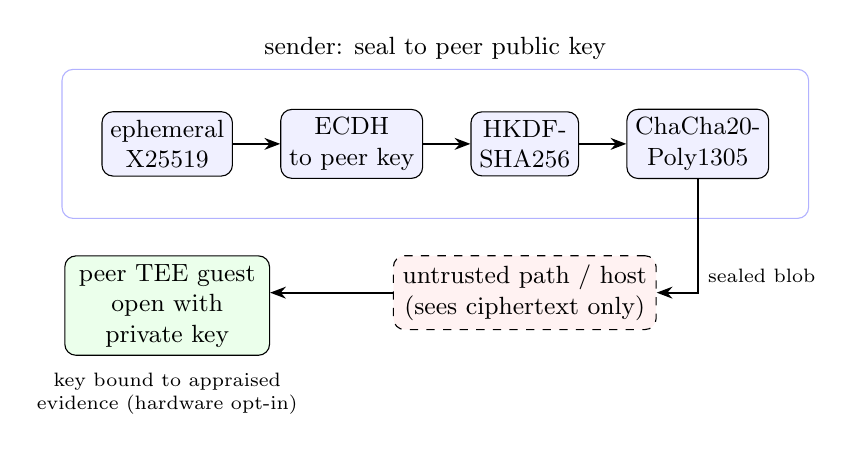
\begin{tikzpicture}[
  font=\small,
  node distance=6mm,
  cryptobox/.style={draw, rounded corners, minimum height=8mm, align=center,
    fill=blue!6, inner sep=3pt},
  enclavebox/.style={draw, rounded corners, minimum height=8mm, align=center,
    fill=green!8, inner sep=3pt},
  flow/.style={-{Stealth[length=2mm]}, thick},
]
  % Sender-side derivation pipeline.
  \node[cryptobox] (eph) {ephemeral\\X25519};
  \node[cryptobox, right=of eph] (ecdh) {ECDH\\to peer key};
  \node[cryptobox, right=of ecdh] (hkdf) {HKDF-\\SHA256};
  \node[cryptobox, right=of hkdf] (aead) {ChaCha20-\\Poly1305};
  \draw[flow] (eph) -- (ecdh);
  \draw[flow] (ecdh) -- (hkdf);
  \draw[flow] (hkdf) -- (aead);

  % Untrusted path carrying ciphertext.
  \node[draw, dashed, rounded corners, below=10mm of hkdf, minimum width=32mm,
    minimum height=7mm, align=center, fill=red!5] (wire)
    {untrusted path / host\\(sees ciphertext only)};
  \draw[flow] (aead.south) |- (wire.east) node[midway, above right, font=\scriptsize]
    {sealed blob};

  % Peer enclave that opens the blob.
  \node[enclavebox, below=10mm of eph, minimum width=26mm] (peer)
    {peer TEE guest\\open with\\private key};
  \draw[flow] (wire.west) -- (wire.west -| peer.east);
  \node[below=1mm of peer, font=\scriptsize, align=center]
    {key bound to appraised\\evidence (hardware opt-in)};

  % Grouping label for the sender pipeline.
  \begin{scope}[on background layer]
    \node[draw=blue!30, rounded corners, fit=(eph)(aead), inner sep=5mm,
      label=above:{sender: seal to peer public key}] {};
  \end{scope}
\end{tikzpicture}
\caption{Sealed peer channel. An ephemeral X25519 ECDH to the peer's channel key is run
through HKDF-SHA256 to derive a symmetric key, and the payload is sealed under
ChaCha20-Poly1305 AEAD. The untrusted connectivity path sees only ciphertext; only the
private key matching the appraised channel key opens the blob. Whether the peer's host can
reach that key depends on the platform (Section~\ref{sec:after}).}
\label{fig:sealed-channel}
\end{figure}

\subsection{Primitive 4: provenance DAG}\label{subsec:provenance}

cA2A emits a signed TRACE record per delegation hop \citep{trace2025}. The A2A profile adds a
delegation-link block to the base TRACE record, which otherwise carries a subject but no notion
of a parent. The block has \texttt{delegation.parent\_record\_hash}, the hash of the parent
hop's TRACE record, and \texttt{delegation.credential\_id}, the id of the delegation credential
this hop acted under. A root hop omits the block; each subsequent hop references its parent, so
the set of records across A~to~B~to~C reconstructs the delegation tree. The construction follows
the W3C PROV data model \citep{prov2013} for lineage and the SCITT \citep{scitt2024} approach to
transparency over signed statements.

Given the records for a workflow and the recipient's trusted signing keys, a verifier
(\texttt{verify\_trace\_dag}) checks each record's signature and rebuilds the parent links from
\texttt{parent\_record\_hash}; a cross-check (\texttt{cross\_check\_trace\_dag}) then aligns the
path with a separately verified delegation chain, requiring matching path length and credential
identifiers and that each record was signed by the key the chain names as that hop's delegate.
Tampering any signed record breaks its signature, and altering a parent link breaks the chain of
hashes. The runtime also keeps an unsigned \texttt{DelegationRecord} form whose hash links give
only structural consistency: a party able to rewrite the whole path can recompute every link,
so since ca2a 0.3.0 the CLI reports such a path as structurally consistent but not
authenticated. Property~\ref{prop:c5} and Section~\ref{sec:eval-c5} distinguish the two. Both
verifiers accept one ordered root-to-leaf path. The A2A profile's delegation-link block is
defined in trace-spec.

Figure~\ref{fig:delegation-dag} shows both halves together: the attenuated delegation chain
on top, where each hop's scope is a subset of its parent's (strictly smaller in this example), and the hash-linked
provenance path below, where each record carries the hash of its parent record and names the
credential the hop acted under. The two are bound: record $i$ must match credential $i$ and, for
signed records, must be signed by that credential's delegate key.

\begin{figure}[h]
\centering
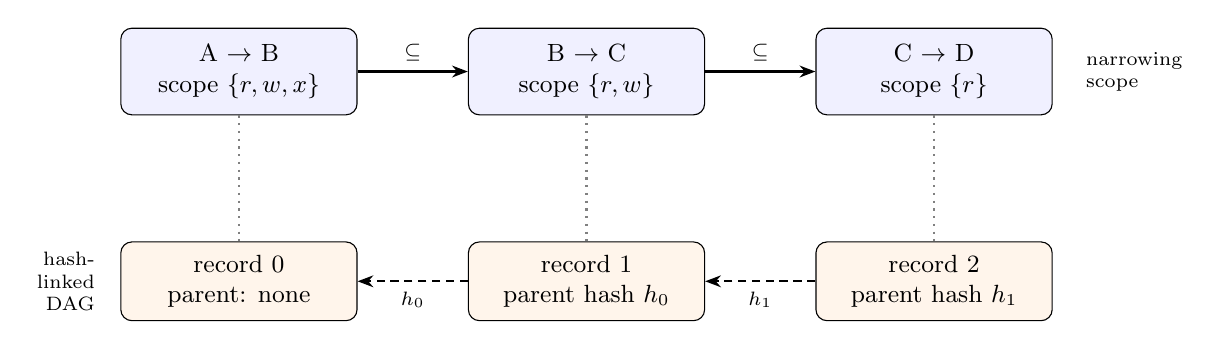
\begin{tikzpicture}[
  font=\small,
  credbox/.style={draw, rounded corners, minimum width=30mm, minimum height=11mm,
    align=center, fill=blue!6, inner sep=2pt},
  recbox/.style={draw, rounded corners, minimum width=30mm, minimum height=10mm,
    align=center, fill=orange!8, inner sep=2pt},
  deleg/.style={-{Stealth[length=2mm]}, thick},
  hashlink/.style={-{Stealth[length=2mm]}, thick, densely dashed},
  bind/.style={dotted, thick, gray},
]
  % Attenuated delegation chain (top row): scope narrows per hop.
  \node[credbox] (a) {A $\to$ B\\scope $\{r,w,x\}$};
  \node[credbox, right=14mm of a] (b) {B $\to$ C\\scope $\{r,w\}$};
  \node[credbox, right=14mm of b] (c) {C $\to$ D\\scope $\{r\}$};
  \draw[deleg] (a) -- node[above, font=\scriptsize] {$\subseteq$} (b);
  \draw[deleg] (b) -- node[above, font=\scriptsize] {$\subseteq$} (c);

  % Provenance records (bottom row), hash-linked to parent.
  \node[recbox, below=16mm of a] (r0) {record 0\\parent: none};
  \node[recbox, below=16mm of b] (r1) {record 1\\parent hash $h_0$};
  \node[recbox, below=16mm of c] (r2) {record 2\\parent hash $h_1$};
  \draw[hashlink] (r1) -- node[below, font=\scriptsize] {$h_0$} (r0);
  \draw[hashlink] (r2) -- node[below, font=\scriptsize] {$h_1$} (r1);

  % Bind record i to credential i.
  \draw[bind] (a) -- (r0);
  \draw[bind] (b) -- (r1);
  \draw[bind] (c) -- (r2);

  \node[right=3mm of c, align=left, font=\scriptsize] {narrowing\\scope};
  \node[left=2mm of r0, align=right, font=\scriptsize] {hash-\\linked\\DAG};
\end{tikzpicture}
\caption{Attenuated delegation chain (top, solid) and its hash-linked provenance DAG
(bottom, dashed). Each delegation hop's scope is a provable subset ($\subseteq$) of its
parent's; each provenance record stores the SHA-256 hash of its parent record. The dotted
lines bind record $i$ to credential $i$. With signed records and trusted keys, tampering,
reparenting, or attributing a record to the wrong delegate is detected offline; hash links
alone give only structural consistency.}
\label{fig:delegation-dag}
\end{figure}

\subsection{Scope-policy intersection}\label{subsec:cedar}

Verifying that a delegated grant is well-formed is not the same as deciding that the local peer
is willing to act on it. On an inbound call, the cA2A runtime is specified to intersect the
delegated scope $S_B$ with the peer's local authorization policy, expressed in Cedar
\citep{cedar2023} or as a simple allow set, and to act only on the intersection
$S_B \cap P_{\text{local}}$. A grant is
thus bounded from above by both the delegator's authority (attenuation) and the delegate's own
policy, so neither a broad grant nor a permissive local default alone can widen what B actually
does.

\textbf{Implementation status.} The intersection runs against either a Cedar engine
(\texttt{cedarpy} 4.8.7) or the set-based \texttt{LocalPolicy}, inside the inbound decision
path (\texttt{handle\_peer\_request}). That path is served by the reference HTTP transport
(since ca2a commit \texttt{7d33445}, July 2026) and by a bridge to the official \texttt{a2a-sdk}
(commit \texttt{f26e2bc}), which the project tests over a local JSON-RPC loopback with
\texttt{a2a-sdk} 1.1.4. Property~\ref{prop:c3} is evaluated in Section~\ref{sec:eval-c3}.

\subsection{Primitives to properties}

Table~\ref{tab:primitives} maps each primitive to the asset it protects, the security property
it supports, and its status at ca2a 0.3.1. The software results need no hardware TEE and can be
rerun from the open-source codebase; the hardware dependencies are stated per row.

\begin{table}[h]
\centering
\caption{cA2A primitives, the assets they protect, the properties they support, and status.
``Validated'' means backed by the rerun software experiments of Section~\ref{sec:evaluation},
at the layer stated.}
\label{tab:primitives}
\small
\begin{tabular}{@{}>{\raggedright\arraybackslash}p{3.0cm}>{\raggedright\arraybackslash}p{3.4cm}>{\raggedright\arraybackslash}p{3.4cm}>{\raggedright\arraybackslash}p{3.4cm}@{}}
\toprule
\textbf{Primitive} & \textbf{Asset protected} & \textbf{Property} & \textbf{Status} \\
\midrule
Attenuated delegation & Bounded authority (no delegate exceeds its grant) &
  C1 attenuation soundness; C2 in-chain replay and splice rejection & Validated (software) \\
Scope-policy intersection & Bounded authority under local policy &
  C3 scope-policy intersection & Validated (software), including the reference inbound path \\
Runtime peer attestation & Peer integrity (only appraised code trusted) &
  C6 cross-operator attestation & Synthetic evidence only; hardware runs one-directional or same-operator \\
Sealed peer channel & Task confidentiality to the intended peer &
  C4 sealed-payload confidentiality & Validated (cryptographic layer); key confinement not shown \\
Provenance record & Provenance (signed record of who delegated what) &
  C5 provenance integrity & Structural checks validated; signed path covered by project tests \\
\bottomrule
\end{tabular}
\end{table}

\section{Security Properties}\label{sec:claims}

We state six security properties of the cA2A profile. Each is an informal invariant over the
runtime; formal proofs are left to future work. Each carries a status line for ca2a 0.3.1 that
names the layer at which it has been checked and what that check does not cover. This section
states the guarantees and mechanisms; results appear in Section~\ref{sec:evaluation}.

\begin{property}[Attenuation Soundness]
\label{prop:c1}
\emph{Status: validated in software.} For any delegation chain of signed credentials rooted at a
trusted issuer, the scope granted at each hop is a subset of the scope of its parent, and any
attempt to grant a capability the parent does not hold is rejected. This is the confused-deputy
defense \citep{confuseddeputy1988} within a chain: without it, a delegate could accept a narrow task and then
act with authority the delegator never conferred. The mechanism is a per-hop subset check in
\texttt{verify\_chain}: each credential carries a \texttt{scope} set, a \texttt{depth}, a
\texttt{parent\_id}, and a detached Ed25519 signature \citep{eddsa2017} over the canonical body.
A hop whose \texttt{scope} is not contained in its parent's \texttt{scope} raises
\texttt{ScopeEscalation}; a monotone-narrowing chain verifies. The semantics mirror
agent-manifest \citep{agentmanifest2026} and follow the capability-attenuation model of
macaroons \citep{macaroons2014}.
\end{property}

\begin{property}[In-Chain Replay and Splice Rejection]
\label{prop:c2}
\emph{Status: validated in software.} A credential presented twice within a chain, or lifted
from one chain and spliced into another, is rejected. This forecloses splicing a legitimately
issued grant into an unrelated delegation to inherit authority out of context. The mechanism
combines two checks in \texttt{verify\_chain}. First, each hop's \texttt{credential\_id} must be
unique within the chain; a repeat raises \texttt{CredentialReplay}. Second, structural
continuity binds each hop to the previous one: a hop's \texttt{parent\_id} must equal the
previous hop's \texttt{credential\_id} and its \texttt{issuer} must equal the previous hop's
\texttt{subject}. A credential spliced from a foreign chain breaks one of these links and raises
\texttt{BrokenDelegationLink}. The property does not cover presentation of a whole valid chain
by a party other than its delegate, since the verifier keeps no global history; on the live path
that case is refused by the holder proof (Section~\ref{sec:after}). Nor does it cover the delegate
itself presenting a valid chain with a request from a different task, since nothing binds a
chain to an execution (Section~\ref{sec:design}).
\end{property}

\begin{property}[Scope-Policy Intersection]
\label{prop:c3}
\emph{Status: validated in software, including the inbound path of the reference transport.}
The effective permission at an inbound peer call is the delegated scope intersected with the
receiving agent's local policy \citep{cedar2023}: a capability is exercised only if the upstream
chain granted it \emph{and} the local policy independently permits it. This makes each domain the
final authority over what runs on its own resources, so an over-broad delegated grant cannot force
action the receiver's policy forbids. The mechanism is the intersection of the verified chain
scope (Property~\ref{prop:c1}) with the local policy decision, evaluated in
\texttt{effective\_scope} and \texttt{enforce\_peer\_call} in \texttt{ca2a\_runtime.peer}; a
capability outside the intersection raises \texttt{ScopeNotPermitted}. Local policy is either a
Cedar policy set evaluated by \texttt{cedarpy} or a set-based \texttt{LocalPolicy}. The same
decision runs inside \texttt{handle\_peer\_request}, which the reference HTTP transport and the
\texttt{a2a-sdk} bridge call on each inbound request. The check does not cover third-party A2A
servers or a production deployment.
\end{property}

\begin{property}[Sealed-Payload Confidentiality]
\label{prop:c4}
\emph{Status: validated at the cryptographic layer.} A task payload sent across a trust boundary
decrypts only with the private key matching the channel key the caller appraised, so no party on
the connectivity path can read plaintext. The mechanism seals the payload to the peer's channel
public key with an HPKE-style X25519, HKDF-SHA256, and ChaCha20-Poly1305 construction
(\texttt{ca2a\_runtime.channel}); only the peer's private key opens it, an unrelated key fails,
and a tampered ciphertext fails closed under AEAD authentication. What software cannot establish
is that the private key is confined to the attested code, so that the operator hosting the peer
cannot read it. That depends on hardware appraisal being required on the call, on the
measurement covering the code that holds the key, and on platform protections such as SEV-SNP
ciphertext hiding. Section~\ref{sec:after} records that the measured hosts did not meet the last
two conditions. Until they are met, confidential payloads should not be sent across a trust
boundary in the belief that a compromised host cannot read them.
\end{property}

\begin{property}[Provenance Integrity]
\label{prop:c5}
\emph{Status: structural checks validated in software; authenticated lineage covered by the
project's tests.} The per-hop records for a workflow form a linked path that is bound to the
delegation authority. With signed TRACE records and trusted signing keys, tampering with any
record, reparenting a record, or attributing a record to a hop that did not sign it is detected
offline \citep{prov2013}. The mechanism adds a delegation-link block to each record:
\texttt{parent\_record\_hash} links a hop to its parent, and \texttt{credential\_id} names the
credential the hop acted under. Altering a record changes its hash and breaks the child's
\texttt{parent\_record\_hash} link, raising \texttt{ProvenanceLinkBroken}. A cross-check binds the
provenance path to the delegation chain of Property~\ref{prop:c1}: record $i$ must correspond to
credential $i$, and a signed record must carry the delegate key that credential names. Hash links
without signatures detect only partial edits: a writer who rewrites the whole path can recompute
every link. The property does not establish that declared work completed or that the submitted
path is complete.
\end{property}

\begin{property}[Cross-Operator Attestation]
\label{prop:c6}
\emph{Status: exercised with synthetic evidence; not validated on hardware across independent
operators.} Two agents in independent trust domains, holding independently generated keys, each
appraise the other's runtime attestation before a delegated task is accepted, and a peer that
loads a different binary than the one expected is detected. The mechanism follows the IETF RATS
architecture \citep{rats2021}: each peer produces a hardware-signed attestation report binding its
channel key and a nonce, and the counterpart verifies the report's certificate chain and
signature and compares its measurement with an expected value, so a binary swap changes the
measurement and is rejected. The SEV-SNP, TDX, and TPM verifiers that this requires ship in ca2a
0.3.1 (Section~\ref{subsec:attestation}). The recorded hardware runs are one-directional across
two clouds, or mutual within one operator's project; neither is mutual attestation between
independent operators.
\end{property}

\section{Evaluation}\label{sec:evaluation}

We evaluate the six properties of Section~\ref{sec:claims} against ca2a 0.3.1, then the current
release (commit \texttt{7d90823}, September 26, 2026); 0.4.0 followed on October 1, 2026
(Section~\ref{sec:after}). Every experiment in this section was rerun
on September 27, 2026. The original July 2026 results came from an earlier, unpinned checkout;
where numbers changed, both are reported.

\subsection{Environment and reproducibility}

The experiments ran under CPython 3.12.10 (an x86-64 build running under emulation on a Windows
11 laptop with an ARM64 Snapdragon X1E80100 processor), with dependencies from the project's
runtime lock at that commit: \texttt{cryptography} 50.0.1, \texttt{cedarpy} 4.8.7,
\texttt{agent-manifest} 0.12.0, \texttt{agentrust-trace} 0.10.0, and \texttt{rfc8785} 0.1.4. The
one deviation from the lock is \texttt{cbor2} 5.9.0 in place of 6.1.4, because the host's
application-control policy blocks the 6.x native extension. Timings are single runs under
emulation and vary from run to run; they show how cost scales, not what a server would measure.
No hardware TEE is needed. The rerun record, with every command's output, is committed with the
paper as \texttt{experiments/results/rerun-2026-09-27.txt}.

Two sets of experiments are used. The repository's own per-claim experiments live under
\texttt{experiments/} in ca2a~\citep{ca2arepo2026}; the three scale and cost experiments below
ship with this report and import the runtime from a ca2a checkout named by \texttt{CA2A\_ROOT}:

\begin{lstlisting}[language=bash,caption={Rerunning the experiments}]
# in a ca2a checkout at tag v0.3.1
pip install -e ".[dev]"
python experiments/claim1-attenuation-soundness/run.py   # C1 .. claim6 likewise
# in this report's directory
CA2A_ROOT=/path/to/ca2a python experiments/c1_attenuation_scale.py
CA2A_ROOT=/path/to/ca2a python experiments/verify_latency_vs_depth.py
CA2A_ROOT=/path/to/ca2a python experiments/sealed_channel_throughput.py
\end{lstlisting}

At 0.3.1, \texttt{verify\_chain} refuses a chain whose root issuer the caller has not named as
trusted (ca2a commit \texttt{23c980a}), so the three report scripts now pass each chain's root as
the trusted set; no other logic changed. The project's test suite at the same commit produced 779
passes and 11 skips: nine skips need a git checkout rather than the source archive used here, and
two need hardware captures. Setting \texttt{CA2A\_TDX\_QUOTE} to a genuine GCP Intel TDX quote
published in the agent-manifest repository ran one of those two: the TDX verifier appraised it to
the pinned Intel SGX Root CA, and all 17 TDX tests passed. That is offline appraisal of one
captured quote, not a live attested call. Table~\ref{tab:ca2a-results} summarizes the outcomes.

\begin{table}[h]
\centering
\caption{Outcomes at ca2a 0.3.1, rerun September 27, 2026. The Status column names the layer at
which each property was checked.}
\label{tab:ca2a-results}
\small
\begin{tabular}{>{\raggedright\arraybackslash}p{3.3cm}>{\raggedright\arraybackslash}p{2.6cm}>{\raggedright\arraybackslash}p{8.2cm}}
\toprule
Property & Status & Result \\
\midrule
C1 Attenuation soundness & Validated (software) & 200/200 narrowing chains accepted and 200/200 escalations rejected with \texttt{ScopeEscalation}; across depths 2 to 8, 2500/2500 accepted and 2500/2500 rejected \\
C2 In-chain replay and splice & Validated (software) & Duplicate \texttt{credential\_id} raises \texttt{CredentialReplay}; cross-chain splice raises \texttt{BrokenDelegationLink}; 2/2 controls valid \\
C3 Scope-policy intersection & Validated (software) & Effective scope is delegated $\cap$ local policy; 1/1 allowed, 3/3 denied; the inbound transport tests exercise the same decision \\
C4 Sealed-payload confidentiality & Cryptographic layer & 4/4: only the peer's key opens the payload; the path sees ciphertext; wrong key and tamper fail closed. Key confinement to attested code not shown \\
C5 Provenance integrity & Structural (experiment) & Tampering one record changed 119 and 138 of 256 hash bits in two runs and raised \texttt{ProvenanceLinkBroken}; reparenting detected; record $i$ bound to credential $i$ \\
C6 Cross-operator attestation & Synthetic evidence & 4/4 with synthetic SEV-SNP vectors: independent keys, mutual appraisal, sealed delegation, binary swap rejected. No hardware run across independent operators \\
\bottomrule
\end{tabular}
\end{table}

\subsection{C1: Attenuation Soundness}
\label{sec:eval-c1}

\textbf{Setup.} Property~\ref{prop:c1} states that a child grant can never exceed its parent.
The repository experiment generates 200 independent four-hop delegation chains. In the narrowing
case, each hop drops exactly one capability from a six-capability root, so every hop is a strict
subset of the one above it. In the escalating case, the third hop adds a fresh capability that no
ancestor held. Each chain is signed hop by hop, so issuer continuity, depth, and
\texttt{parent\_id} linkage hold; only the scope relationship differs.

\textbf{Results.} All 200 narrowing chains are accepted, and all 200 escalating chains are
rejected with \texttt{ScopeEscalation}; none is rejected by an unrelated error. A correctly
signed credential that widens its scope is still rejected, so attenuation is enforced
independently of signature validity.

\textbf{Across chain depth.} For each depth in $\{2,3,4,6,8\}$ we generated 500 narrowing chains
and 500 escalation chains (each escalation injects a never-held capability at an interior hop)
over a 16-capability root universe, 2500 of each in total. Every narrowing chain was accepted and
every escalation was rejected with \texttt{ScopeEscalation}, with zero rejections by an unrelated
error, matching the July result. The per-depth counts are in
\texttt{experiments/results/c1\_attenuation\_scale.json}.

\subsection{Verification Latency vs Chain Depth}
\label{sec:eval-latency}

\textbf{Setup.} Chain verification is the per-call cost a callee pays before it acts: trusted
root, signature, validity, continuity, attenuation, and in-chain replay over every hop. We built
one correctly signed chain at each depth in $\{1,2,4,8,16,32,64\}$, ran 200 warm-up iterations,
then timed \texttt{verify\_chain} over 2000 iterations per depth, reporting mean, p50, and p99.
Chains are signed once up front, so the measurement excludes key generation.

\textbf{Results.} Cost grows linearly with depth, at about 216 microseconds per hop between depth
1 and depth 64 (July: about 195). A single hop verifies in 0.25\,ms mean; a 64-hop chain verifies
in 13.87\,ms mean with p99 26.08\,ms (July: 0.14\,ms, 12.45\,ms, and 22.15\,ms).
Table~\ref{tab:rerun-compare} lists both runs, and Figure~\ref{fig:latency-depth} plots the rerun.
The two runs differ in code version (the verifier gained trusted-root and validity-window checks
after July) and in environment, so the difference is not attributed to either alone. At realistic depths of a few
hops the cost stays near a millisecond or below. Raw values are in
\texttt{experiments/results/verify\_latency\_vs\_depth.json}.

\begin{table}[h]
\centering
\caption{Original (July 1, 2026, unpinned checkout) and rerun (September 27, 2026, ca2a 0.3.1)
timings. Both are single runs on developer hardware.}
\label{tab:rerun-compare}
\small
\begin{tabular}{lrr}
\toprule
Measurement & July 2026 & Rerun \\
\midrule
\texttt{verify\_chain}, depth 1, mean (ms) & 0.14 & 0.25 \\
\texttt{verify\_chain}, depth 8, mean (ms) & 1.73 & 2.07 \\
\texttt{verify\_chain}, depth 64, mean / p99 (ms) & 12.45 / 22.15 & 13.87 / 26.08 \\
Slope, depth 1 to 64 ($\mu$s per hop) & 195 & 216 \\
Seal and open, 64 bytes, round trip (ms) & 0.21 & 0.17 \\
Seal and open, 256\,KiB, throughput (MiB/s) & 266 & 212 \\
\bottomrule
\end{tabular}
\end{table}

\begin{figure}[h]
\centering
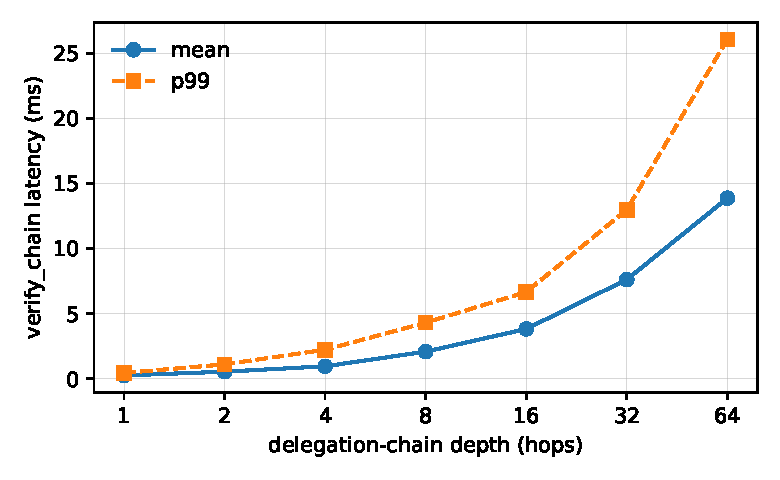
\includegraphics[width=0.62\linewidth]{figures/verify_latency_vs_depth.pdf}
\caption{Chain-verification latency (mean and p99) versus delegation-chain depth, log-scale
x-axis, 2000 timed iterations per depth, ca2a 0.3.1. Cost is linear in depth at about 216
microseconds per hop; a 64-hop chain verifies in 13.87\,ms mean.}
\label{fig:latency-depth}
\end{figure}

\subsection{C2: In-Chain Replay and Splice Rejection}
\label{sec:eval-c2}

\textbf{Setup.} Property~\ref{prop:c2} states that a credential replayed within a chain or
spliced from another chain is rejected. We build two independent, well-formed chains, A and B,
each with its own key material and credential-id namespace. Three cases are checked: (1) a
control in which both chains verify unmodified; (2) an intra-chain replay in which one hop's
\texttt{credential\_id} is duplicated inside the chain; and (3) a cross-chain splice in which a
validly signed credential minted for chain A is inserted into chain B.

\textbf{Results.} Both control chains verify (2/2). The duplicated \texttt{credential\_id} raises
\texttt{CredentialReplay}. The spliced credential is rejected with \texttt{BrokenDelegationLink}
because its \texttt{parent\_id} does not match chain B's preceding credential. A valid signature is
therefore necessary but not sufficient; continuity is enforced over the chain, not per
credential. Replay of a whole valid chain by a different party is outside this experiment; the
project covers it with holder-proof tests.

\subsection{C3: Scope-Policy Intersection}
\label{sec:eval-c3}

\textbf{Setup.} Property~\ref{prop:c3} states that the capability a caller may exercise against a
peer is the intersection of its verified delegated scope with the callee's local policy. We build
a two-hop chain delegating a leaf scope of \{\texttt{read}, \texttt{write}\} (the root also held
\texttt{admin}) and set the callee's local policy to allow \{\texttt{read}, \texttt{audit}\}. We
then request four capabilities through \texttt{effective\_scope} and \texttt{enforce\_peer\_call}:
\texttt{read} (delegated and allowed), \texttt{write} (delegated but not locally allowed),
\texttt{audit} (locally allowed but never delegated), and \texttt{admin} (neither).

\textbf{Results.} The effective scope is exactly \{\texttt{read}\}. Only \texttt{read} is allowed
(1/1); \texttt{write}, \texttt{audit}, and \texttt{admin} are each denied with
\texttt{ScopeNotPermitted} (3/3). A capability is exercised only when the chain granted it
\emph{and} the local policy permits it. The experiment uses the set-based \texttt{LocalPolicy};
the project's unit tests exercise the Cedar engine, and its live-call and \texttt{a2a-sdk}
loopback tests, which passed in the rerun, drive the same decision through an inbound HTTP and
JSON-RPC request on the local host, including a denial for an out-of-scope capability. None of
these is a deployment across a real network boundary.

\subsection{C4: Sealed-Payload Confidentiality}
\label{sec:eval-c4}

\textbf{Setup.} Property~\ref{prop:c4} states that a sealed task payload decrypts only with the
private key matching the peer's appraised channel key. The peer generates a channel keypair; we
seal a secret payload to its public key with \texttt{ca2a\_runtime.channel} and check four
sub-properties: (1) the sealed blob does not contain the plaintext; (2) the peer's private key
recovers it; (3) an unrelated key cannot open it; and (4) a tampered ciphertext fails closed
under AEAD authentication.

\textbf{Results.} All four checks pass (4/4). A different key and a flipped byte both raise
\texttt{SealedChannelError} rather than returning corrupted plaintext. This validates payload
confidentiality at the cryptographic layer. It says nothing about whether the peer's host can read
the private key; that is the hardware dependency Property~\ref{prop:c4} names, and
Section~\ref{sec:after} reports platform state that bears on it.

\textbf{Throughput and latency.} We measured the sealed channel across payload sizes from a
64-byte task envelope to a 256\,KiB document, timing \texttt{seal} (ephemeral key generation,
ECDH, HKDF, AEAD encryption) and \texttt{open} (ECDH, HKDF, AEAD decryption) over 2000 iterations
each after warm-up, with a round-trip check confirming every opened payload equalled the
original. A 64-byte envelope seals and opens in 0.17\,ms round trip, a cost dominated by the fixed
X25519 and HKDF setup. As payloads grow the setup amortizes and the AEAD dominates: end-to-end
throughput rises from 0.37\,MiB/s at 64 bytes to 212\,MiB/s at 256\,KiB (July: 0.21\,ms and
266\,MiB/s). Figure~\ref{fig:sealed-throughput} plots the rerun. Raw measurements are in
\texttt{experiments/results/sealed\_channel\_throughput.json}.

\begin{figure}[h]
\centering
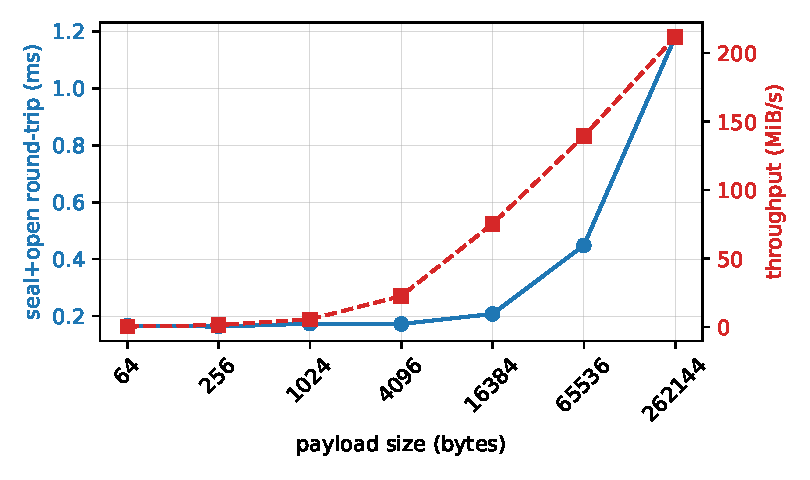
\includegraphics[width=0.64\linewidth]{figures/sealed_channel_throughput.pdf}
\caption{Sealed-channel round-trip latency (left axis) and end-to-end throughput (right axis)
versus payload size, log-scale x-axis, 2000 timed \texttt{seal} and \texttt{open} iterations per
size, ca2a 0.3.1. Small payloads are setup-dominated (0.17\,ms round trip at 64 bytes); large
payloads are AEAD-dominated, reaching 212\,MiB/s at 256\,KiB.}
\label{fig:sealed-throughput}
\end{figure}

\subsection{C5: Provenance Integrity}
\label{sec:eval-c5}

\textbf{Setup.} From a signed three-hop chain the repository experiment emits one unsigned
\texttt{DelegationRecord} per hop, each carrying the SHA-256 \texttt{record\_hash} of its parent.
It checks four sub-properties: (1) a valid record set verifies with \texttt{verify\_dag}; (2)
changing a record's scope changes its \texttt{record\_hash} and breaks its child's parent link;
(3) pointing a record at the wrong ancestor is detected; and (4) \texttt{cross\_check\_chain}
binds record $i$ to credential $i$.

\textbf{Results.} The valid record set verifies. Injecting one capability into a record's scope
changed 119 and 138 of the 256 bits of its \texttt{record\_hash} in two runs, as expected of
SHA-256~\citep{avalanche1985}, and \texttt{verify\_dag} raised \texttt{ProvenanceLinkBroken}
because the child's stored parent hash no longer matched. Reparenting the leaf record was likewise
detected, and \texttt{cross\_check\_chain} raised \texttt{ProvenanceLinkBroken} when a record's
\texttt{credential\_id} was forged.

\textbf{What this shows.} These records are unsigned, so the experiment shows structural
consistency against a single edit, not authenticity: a writer who rewrites every record can
recompute every link and pass all four checks, and an edit to the leaf has no child link to
break. Authenticity comes from the signed TRACE path (\texttt{verify\_trace\_dag} and
\texttt{cross\_check\_trace\_dag}), whose unit tests, including those binding each record's
signing key to the chain's delegate, passed in the rerun. That path is not measured by a separate
experiment in this report.

\subsection{C6: Cross-Operator Attestation}
\label{sec:eval-c6}

\textbf{Setup.} The repository experiment builds two operators, each with its own channel keypair
and its own synthetic VCEK key, and binds each channel key into a synthetic SEV-SNP report. Both
synthetic VCEK certificates chain to one synthetic root standing in for the AMD ARK. Each side
verifies the other's report chain and signature with the shipped verifier, checks the
measurement against an expected value, seals a delegated task to the key the report binds, and
finally presents a validly signed report with a different measurement.

\textbf{Results.} All four checks pass (4/4): the keys are independent, each report's channel key
is recovered after verification, the sealed task opens only with the peer's key, and the report
with the swapped measurement is rejected with \texttt{AttestationFailed}. This exercises the
protocol logic and the verifier code. It does not show that genuine hardware produces such
reports for this protocol between independent operators. The recorded hardware runs
(Section~\ref{subsec:attestation}) were one-directional across two clouds or mutual within one
operator, their raw evidence is not published, and they were not repeated for this edition. C6
therefore remains unvalidated on hardware.

\section{Findings after the evaluation}\label{sec:after}

The July 2026 draft was evaluated against an early checkout. Later work in the ca2a repository
found gaps in that code and in the draft's claims. They are listed here with the commit that
addressed each and the first release containing it, so that the July results can be read against
them. All are recorded in the project's changelog.

\textbf{A delegation chain was a bearer credential.} The inbound path verified a chain and then
granted its leaf authority without asking the caller to show any relationship to the leaf
subject, so anyone holding a copy of a published chain could exercise it, and the provenance
record would name the legitimate delegate. Property~\ref{prop:c2} as tested does not catch this,
because nothing inside the chain changes. Since commit \texttt{cbfeb40} (0.2.0) the callee issues
a challenge and requires a signature under the leaf subject's key over the request, the channel
key, and the payload digest.

\textbf{Untrusted roots were accepted.} A chain that was internally consistent verified whoever
minted its root, so an attacker could grant itself any locally allowed capability (GHSA-95qh-qjph-8622). The runtime
required a trusted root set from commit \texttt{e647e90} (0.2.0), and \texttt{verify\_chain}
itself from commit \texttt{23c980a} (0.3.0). The July C1 and C2 results were produced without a
trust set; the rerun supplies one.

\textbf{Unsigned provenance did not authenticate lineage.} The July draft described the C5 records
as verifiable ``from signed records alone'', but the experiment used unsigned records whose hash
links a writer can recompute. Since commit \texttt{550fba9} (0.3.0) the CLI separates
authenticated lineage over signed TRACE records from structural diagnostics, and commit
\texttt{e8b5cb7} (0.3.0) requires each signed record's key to match the delegate named by the
chain, which the cross-check had not compared.

\textbf{Grants could not be revoked early.} Until commit \texttt{f018c0e} (0.3.0) a credential
stayed valid for its whole window. Issuers can now sign revocation statements that a verifier
consults through a supplied snapshot. cA2A does not publish or fetch revocation data, and a
verifier without a snapshot reports revocation as not checked.

\textbf{The TDX parser rejected every genuine quote.} Real DCAP v4 quotes nest the quoting-enclave
data under a type-6 header that the parser and its synthetic fixtures both omitted, so the TDX
path had never accepted real evidence. The failure was closed rather than an unsound accept. It
was fixed in commit \texttt{82be440} (0.2.0) when a genuine quote was first appraised, which is
why this edition re-appraised a public genuine quote rather than relying on synthetic vectors.

\textbf{Measured hosts lacked platform protections.} The GCP SEV-SNP hosts used on August 24 and
September 17, 2026 reported \texttt{PLATFORM\_INFO} 0x25: SMT enabled and ciphertext hiding not
enabled. Stricter platform policies correctly refused them. cA2A can enforce such a policy, but
appraisal of platform state is opt in and off by default. In the September 17 diagnostic the
launch measurement also did not cover application code installed after boot. Both bear directly
on Property~\ref{prop:c4}: a hardware-appraised channel key on such a host is not shown to be out
of the host operator's reach.

\textbf{Malformed input escaped as exceptions.} Before commit \texttt{66ad9f0} (0.3.1) some
malformed wire documents, TDX quotes, and MAC strings raised Python exceptions instead of the
documented error, and the canonicalizer coerced non-string keys so that two distinct objects could
serialize alike. Each now fails with a documented error.

\textbf{Caller attestation could be relayed.} Through 0.3.1 a callee that required hardware
caller attestation appraised the caller's offer but never asked the caller to prove it held the
offered channel key, and any node attested its own key under whatever nonce reached its public
channel endpoint. A delegate with no TEE could fetch an honest hardware peer's offer under the
callee's challenge, present it as its own, and be recorded with hardware caller attestation
(GHSA-xxj2-p57x-x954, affecting 0.2.0 to 0.3.1). Since commit \texttt{19407fb} (0.4.0) caller and
callee offers are signed under separate role prefixes, and the caller sends a MAC keyed from
X25519 between its attested channel key and the callee's. The September 17 diagnostic predates
this fix; it ran honest nodes under one operator, so no relay was attempted, but its caller
appraisal did not include proof of possession. The software experiments of
Section~\ref{sec:evaluation} do not send caller offers, and the six repository experiments
produce the same results at 0.4.0.

\section{Related Work}\label{sec:related}

cA2A draws on three lines of work: capability-based delegation, identity and transparency
standards, and confidential computing for agents. Several of its mechanisms appear in prior or
concurrent work, and we do not claim priority for attenuation or for binding provenance to
authority. What we did not find in the work below is the combination of per-hop attenuation with
appraisal of the delegate's TEE evidence and sealing of the task payload to the key that
evidence vouches for, on the A2A delegation edge.

\paragraph{Capability delegation for agents.}
Macaroons~\citep{macaroons2014} introduced contextual caveats that attenuate a bearer credential
without a round trip to the issuer; a derived credential can only be narrower, and the check is
offline. Toma\v{s}ev, Franklin, and Osindero propose delegation capability tokens for AI agents based
on macaroons or Biscuit tokens, wrapping resource credentials in attenuating
caveats~\citep{tomasev2026}. Prakash's Agent Identity Protocol (AIP) implements invocation-bound
capability tokens that combine identity, attenuated authorization, and provenance in an
append-only token chain, with Biscuit and Datalog policies for multi-hop delegation, bindings for
MCP, A2A, and HTTP, and interoperable Python and Rust implementations~\citep{aip2026}. The PEDIGREE
Internet-Draft, an individual submission from Glyphzero Labs that extends the SPIFFE and WIMSE
workload-identity model, specifies per-hop delegation with scope attenuation enforced at mint and
at verification, Cedar-policy mandates with static-analysis proofs that a child mandate narrows
its parent, and cryptographic re-verification of each parent token to resist parent-swap
attacks~\citep{pedigree2026}. These cover the attenuation and chain-integrity ground of
Properties~\ref{prop:c1} and~\ref{prop:c2}, and PEDIGREE's narrowing proofs over Cedar policies go
further than cA2A's set-subset check. Neither AIP nor PEDIGREE addresses appraisal of the
delegate's runtime attestation or encryption of the task payload to the delegate. cA2A's
delegation semantics mirror agent-manifest~\citep{agentmanifest2026}.

\paragraph{Identity and transparency standards.}
The IETF WIMSE architecture draft~\citep{wimse2025} describes how workloads present and verify
identity across systems, and the SCITT architecture, published as RFC~9943 in June
2026~\citep{scitt2024}, defines transparency services for signed supply-chain statements. The same
author as PEDIGREE has proposed binding per-action authorization and memory provenance into SCITT
agent action capsules~\citep{capsule2026}. cA2A's per-hop records follow the SCITT pattern of
signed statements that a verifier can appraise offline, and the TRACE record format it
emits~\citep{trace2025} has a transparency field that can carry a SCITT receipt; cA2A does not
itself operate a transparency service. From the adversary side, Anbiaee et al.\ compare the security of
MCP, A2A, Agora, and ANP and identify protocol-level and cross-protocol risks, including missing
validation and attestation of executable components~\citep{crossprotocol2026}.

\paragraph{Agent identity and messaging infrastructure.}
AGNTCY, initiated by Cisco and hosted by the Linux Foundation since July 2025, provides agent
discovery, identity, and messaging components for multi-agent systems~\citep{agntcy2026}. It
addresses naming, discovery, and authenticated communication at a scale cA2A does not attempt. We
did not find in its published components a mechanism that intersects a delegated scope with the
receiver's local policy or seals a payload to an appraised TEE key. The two could compose: such a
layer can name the peers while cA2A governs the authority that flows between them.

\paragraph{Hardware-attested provenance.}
EQTY Lab's Verifiable Compute uses TEE attestation to notarize AI computation, pairing Intel TDX
CPUs with NVIDIA H100 GPUs in its published design~\citep{eqtyvc2024}, and its Verifiable
Knowledge work extends that approach to the provenance of data an agent uses, on NVIDIA BlueField
hardware~\citep{eqty2026}. These are commercial systems built around particular hardware pairings.
cA2A's verifier follows the RATS role separation~\citep{rats2021} and appraises SEV-SNP, TDX, and
TPM evidence through one interface, but it has not been validated across independent operators
(Property~\ref{prop:c6}).

\paragraph{Confidential agentic AI.}
Forough, Kogias, and Haddadi survey confidential computing for agentic AI across six TEE platforms
and list open challenges, among them compound attestation for multi-hop agent
chains~\citep{secretssurvey2026}; Mo, Tarkhani, and Haddadi systematize confidential computing for
machine learning more broadly~\citep{confai2024}. cA2A's sealed channel
(Property~\ref{prop:c4}) targets the delegation hop, and Section~\ref{sec:after} records why it is
not yet a confidentiality guarantee against a hosting operator. The sibling cMCP
profile~\citep{cmcp2026} applies confidential computing to the single-agent tool-call boundary;
cA2A applies the same TEE provider pattern and Cedar engine to the agent-to-agent boundary.

\section{Conclusion}\label{sec:conclusion}

A2A standardizes how agents discover each other and exchange tasks, but its trust model stops at
the Signed Agent Card. Card verification establishes that a domain owner issued a card. It does
not establish that the peer runs attested code, that a delegating agent holds the authority it
passes on, that the task payload is confidential to the peer, or that there is a record of who
delegated what to whom. cA2A is a trust profile layered on A2A that addresses these with
attenuated delegation, attestation-gated sealing, and signed per-hop provenance, reusing existing
standards rather than defining a new transport~\citep{a2a2026,trace2025}.

Rerun against ca2a 0.3.1, the software results hold. Attenuation was exact across 2,700
narrowing and 2,700 escalating chains; in-chain replay and cross-chain splices were rejected;
delegated scope was intersected with local policy, including on the reference inbound path;
sealed payloads opened only with the peer's key and failed closed on tamper; and edits to linked
provenance records were detected. Chain verification cost about 0.22\,ms per hop in our
environment, and the sealed channel reached 212\,MiB/s at 256\,KiB.

The limits are as important as the results. The provenance experiment shows structural
consistency; authenticity depends on signed records, which the project's tests cover. The sealed
channel is validated at the cryptographic layer only: the measured hosts lacked SEV-SNP ciphertext
hiding, and the launch measurement in the recorded mutual run did not cover application code.
Cross-operator attestation has been exercised with synthetic evidence and, on hardware, only
one-directionally or within one operator. Section~\ref{sec:after} lists defects found after the
original evaluation, including chains that acted as bearer credentials and unsigned provenance
presented as authenticated; each was fixed in a released version.

Until mutual attestation between independent operators is demonstrated on platforms that provide
the needed memory protections, cA2A should not be described as attested across trust domains or as
protecting payloads from a hosting operator. The specification, verifier, and experiments are
available at \url{https://github.com/agentrust-io/ca2a} under the MIT license.


\bibliographystyle{plainnat}
\bibliography{refs}

\end{document}
